\chapter{Introduction}
\label{ch:introduction}


% - Why set of linear equations arise in scientific computing
% - Why some of the matrices are sparse
% - Time and memory complexity of solving linear systems
% - How does permutation help either reducing fill-in, memory or improving parallelism
% - In this work, we focus solely on the permutation problem. We explore existing methods for sparse symmetric matrix reordering. We explore any possible optimizations and parallelization strategies. We look for single thread, multi-thread and distributed memory implementations.
% - We thoroughly evaluate the performance of the different reordering methods and compare them in various qualities for a lot of different matrices.

Sparse linear systems of the form $Ax = b$, where $A \in \mathbb{R}^{n \times n}$ is sparse and symmetric, are ubiquitous in scientific computing. These systems arise naturally across virtually every domain of computational science and engineering, including quantum chemistry, computer graphics, computational fluid dynamics, power networks, machine learning, and optimization. Formally, one may state matrix $A$ is considered sparse when the number of nonzero entries $\text{nnz}(A)$ satisfies $\text{nnz}(A) = O(n)$ rather than $O(n^2)$ as in dense matrices, although a better practical definition is a matrix is sparse if it is advantageous to exploit its zero entries \cite{scott_introduction_2023}.

% The prevalence of sparse matrices stems from a fundamental mathematical property that many physical phenomena exhibit: local interactions—adjacent elements in a discretized domain interact strongly, while distant elements have minimal or no direct coupling.

% \begin{figure}[!h]
%     \centering
%     \begin{subfigure}[b]{0.44\textwidth}
%         \centering
%         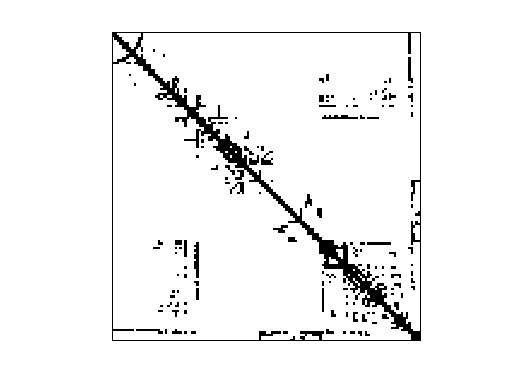
\includegraphics[width=\textwidth]{fig/intro/bcsstk32.png}
%         \caption{Sparsity pattern of the bcsstk32 matrix}
%         \label{fig:bcsstk32-matrix}
%     \end{subfigure}
%     \hfill
%     \begin{subfigure}[b]{0.44\textwidth}
%         \centering
%         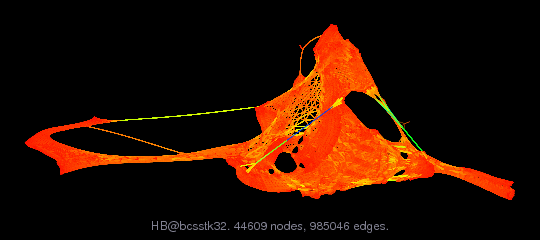
\includegraphics[width=\textwidth]{fig/intro/bcsstk32_graph.png}
%         \caption{Graph representation}
%         \label{fig:bcsstk32-graph}
%     \end{subfigure}
%     \caption{The bcsstk32 matrix from automotive chassis analysis. This 28,924 × 28,924 symmetric matrix represents an automobile chassis structure analyzed using finite element modeling.}
%     \label{fig:bcsstk32-example}
% \end{figure}

 This sparsity typically arises from the discretization of partial differential equations (PDEs) \cite{schaeffer_sparse_2013} using finite difference, finite element, or finite volume methods. When continuous problems described by partial differential equations are discretized using methods such as finite differences, finite elements, or finite volumes, the resulting algebraic equations connect only neighboring (or some specific) grid points or elements. Conceptually, sparsity corresponds to systems with few pairwise interactions. For instance, in a three-dimensional finite element mesh, each node typically connects to only a small neighborhood of adjacent nodes, regardless of the total problem size, resulting in matrices where the number of non-zero elements is roughly equal to the number of rows or columns rather than being proportional to $n^2$.

 Solving sparse linear systems efficiently is critical for the performance. Direct methods such as Cholesky factorization are often employed for such matrices due to their numerical stability and robustness. However, a significant challenge with direct methods is the appearance of fill-ins, where zero entries in the original matrix become non-zero in the factorized form.

\begin{figure}[!h]
    \centering
    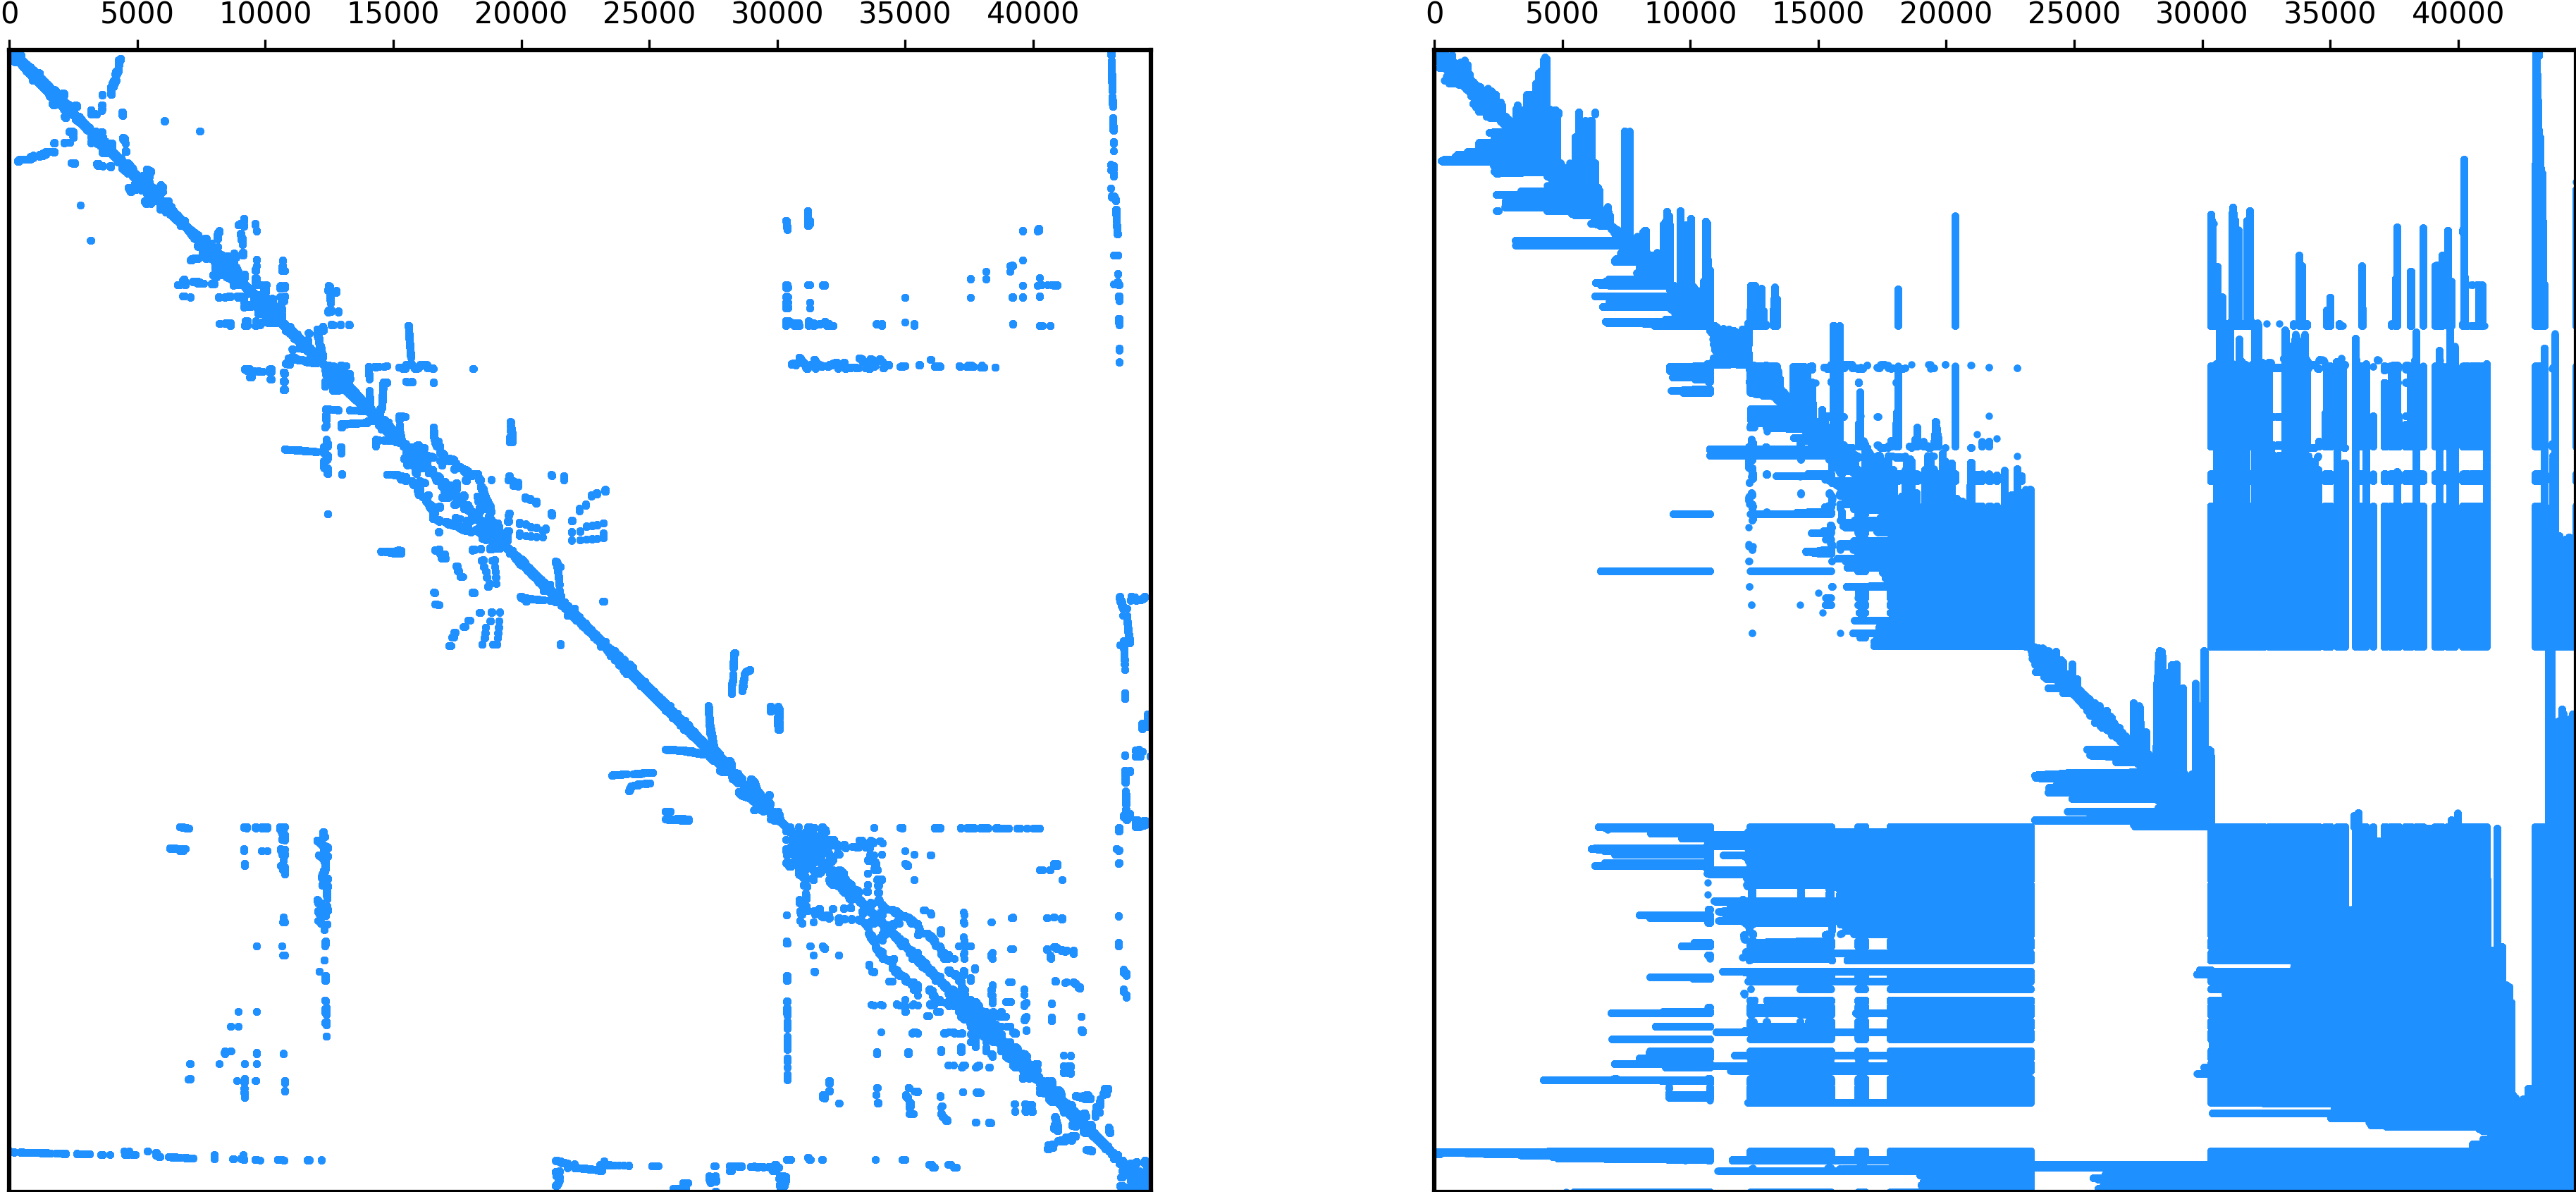
\includegraphics[width=0.9\textwidth]{fig/intro/sparsity_pattern.png}
    \caption{Sparsity pattern of a matrix from structural engineering \texttt{bcsstk32} (left) and \(L+L^T\) (right) where \(L\) is the Cholesky factor of \texttt{bcsstk32}.}
    \label{fig:sparse-matrix-example}
\end{figure}

As we see in \cref{fig:sparse-matrix-example}, the Cholesky factorization of a sparse matrix often results in a denser matrix due to fill-in. This fill-in can significantly increase both memory usage and computational time for solving the system. The amount of fill-in depends on the order in which variables are eliminated during factorization, which is determined by the ordering, or permutation, of the matrix rows and columns. The permutations serve as a preprocessing step that can reduce fill-in largely. The basic principle involves reordering the rows and columns of the matrix $A$ to obtain a permuted system $PAP^T \hat{x} = Pb$, where $P$ is a permutation matrix, such that the reordered matrix exhibits superior properties for factorization. 

In this thesis, we focus exclusively on the permutation problem for sparse symmetric matrices. We explore existing methods for sparse symmetric matrix reordering, investigate potential optimizations and parallelization strategies, and evaluate the performance of different reordering methods across a variety of matrices, assessing their effectiveness in terms of fill-in reduction, memory usage and parallelism. In chapter \ref{ch:background}, we provide the necessary theoretical background on sparse matrix factorization and graph representations. Chapter \ref{ch:implementation_and_optimizations} details the implementation of various reordering algorithms, while Chapter \ref{ch:results} presents an overview of our experimental evaluation. In Chapter \ref{ch:other_approaches}, we discuss other promising approaches that were not fully explored in this work. Finally, Chapter \ref{ch:conclusion} summarizes our findings and suggests directions for future research. For full performance results, please refer to the appendix \ref{app:experimental_results}.


% Consider the solution of a sparse system $Mx = b$, where $M$ is an $n \times n$ symmetric, positive definite matrix. Using Gaussian elimination, we can find the Cholesky factorization $M = LL^T$, where $L$ is a lower triangular matrix with positive diagonal entries. The solution is then obtained by solving two triangular systems: $Ly = b$ and $L^Tx = y$.

% The computational complexity of this procedure depends critically on the sparsity of both $M$ and $L$. If column $j$ of $L$ contains $d\sb{j}$ nonzeros, then the factorization and solution can be performed in space proportional to $\sum\sb{j} d\sb{j}$ (the number of nonzeros in $L$) and time proportional to $\sum\sb{j} d\sb{j}^2$. Ignoring numerical cancellation, $L$ will have nonzeros below the diagonal everywhere that $M$ does, plus additional locations. The \emph{fill} is defined as the set of below-diagonal positions where $L$ is nonzero but $M$ is zero.

% If $P$ is a permutation matrix, then $PMP^T$ represents a reordering of the rows and columns of $M$, and the fill in the triangular factor can vary drastically for different choices of $P$. We can think of $P$ as determining the order in which variables are eliminated from the system.

% Finding the elimination order that minimizes fill is an NP-complete problem. Moreover, most sparse matrices inherently suffer from large fill-in: for any positive $\epsilon$, there exists a constant $c(\epsilon)$ such that almost all $n \times n$ symmetric matrices with $c(\epsilon)n$ nonzeros have at least $(1-\epsilon)n^2/2 - O(n)$ fill for every elimination order. This theoretical limitation underscores why effective heuristic reordering methods are essential.

% The impact of proper ordering can be dramatic in practice: while the Cholesky factorization of an original matrix might result in $L$ having about 8\% nonzero density, appropriate reordering methods can reduce this to less than 1\%. This reduction translates directly to computational savings, potentially reducing factorization cost from $O(n^3)$ to $O(n^{1.5})$ for many practical problems.

% The introduction motivates your work and puts it into a bigger context.
% It should answer the following questions:
% What is the background of this work?
% What is the state of the art?
% Why is this project necessary to advance the state of the art?
% What are the problems that have to be solved and why are they difficult?
% What are your contributions to solve these problems?
% How do you evaluate your solution to show that it is adequate and applicable?

% An introduction written along these questions naturally follows the \textit{\gls{spse}}\footnote{%
%   The \acrshort{spse} approach was established in a book~\cite{Hoey83}, but is also briefly summarized in a more recent article~\cite{MP12}, which is available online.
% } approach.
% In the \emph{situation}, you set the scene for your work and catch the interest of the readers by showing the importance and generality of the scene.
% In the \emph{problem}, you spot an issue in the scene and show why and how it significantly taints the scene.
% In the \emph{solution}, you outline your solution to that issue.
% Finally, in the \emph{evaluation}, you present the main arguments why the claimed solution actually does solve the problem.

% In the following chapters, you will elaborate each of the four \gls{spse} elements in detail:
% In \textsl{Background}, you lay the foundations for an in-depth understanding of the situation and the problem.
% In \textsl{Implementation and Optimizations}, you show how others have address this (or similar) problems and why their solutions are not sufficient or applicable.
% In \textsl{Implementation}, you specify your solution, which you then evaluate rigorously for strengths and weaknesses in \textsl{Results}.

% At the end of the introduction, you should explicitly show this structure to the reader by briefly explaining how this report is organized.
% Instead of using the general \gls{spse} terminology and the chapter names mentioned above, we urge you to use the domain-specific terminology established in the introduction and point to chapters using cross references (e.g., refering to \cref{ch:background} instead of ``the Background chapter'').
